%!TEX program = xelatex
\documentclass[a4paper,UTF8]{ctexart}
\usepackage[unicode=true,colorlinks,linkcolor=blue,bookmarksnumbered=true]{hyperref}
\usepackage{latexsym,amssymb,amsmath,amsbsy,amsopn,amstext,amsthm,amsxtra,color,multicol,bm,calc,ifpdf}
\usepackage{graphicx}
\usepackage{diagbox}   % 绘制表格斜线
\usepackage{enumerate}
\usepackage{epstopdf}
\usepackage{fancyhdr}
\usepackage{subfigure}
\usepackage{listings}
\usepackage{multirow}
\usepackage{makeidx}
\usepackage{xcolor} 
\usepackage{fontspec}                            % 建立索引宏包
\graphicspath{{figures/}}  % 设置图片搜索路径
\theoremstyle{plain} \newtheorem{theorem}{定理}[section]
\theoremstyle{plain} \newtheorem{definition}{定义}[section]
\theoremstyle{plain} \newtheorem{lemma}{引理}[section]
\theoremstyle{plain} \newtheorem{proposition}{命题}[section]
\theoremstyle{plain} \newtheorem{example}{例}[section]
\theoremstyle{plain} \newtheorem{remark}{注}[section]
\theoremstyle{plain} \newtheorem{corollary}{推论}[section]
\newfontfamily\courier{Courier New}
\lstset{linewidth=1.1\textwidth,
        numbers=left, %设置行号位置 
        basicstyle=\small\courier,
        numberstyle=\tiny\courier, %设置行号大小  
        keywordstyle=\color{blue}\courier, %设置关键字颜色  
        %identifierstyle=\bf,
        commentstyle=\it\color[cmyk]{1,0,1,0}\courier, %设置注释颜色 
        stringstyle=\it\color[RGB]{128,0,0}\courier,
        %framexleftmargin=10mm,
        frame=single, %设置边框格式  
        backgroundcolor=\color[RGB]{245,245,244},
        %escapeinside=``, %逃逸字符(1左面的键),用于显示中文  
        breaklines, %自动折行  
        extendedchars=false, %解决代码跨页时,章节标题,页眉等汉字不显示的问题  
        xleftmargin=2em,xrightmargin=2em, aboveskip=1em, %设置边距  
        tabsize=4, %设置tab空格数  
        showspaces=false %不显示空格  
        basicstyle=\small\courier
       }  
\newenvironment{mysolution}{{\color{blue} 解}: }{{\color{magenta}\qed}}
\newcommand\diff{\,{\mathrm d}} %定义微分d
\newcommand{\p}[3]{\frac{\partial^{#1}#2}{\partial{#3}^{#1}}}  %定义求偏导算子
\newcommand{\ucite}[1]{\textsuperscript{\cite{#1}}}  %参考文献引用:上标用\ucite{ },文中用\cite{ }

\begin{document}
\title{

\includegraphics[width=0.65\textwidth]{onepiece.pdf}\\
\vspace{2em}
\textbf{线性回归学习笔记}}
\author{\emph{李向阳}  \color{blue}{d1142845997@gmail.com}
}
\date{}

\maketitle
\thispagestyle{empty}

\newpage


\tableofcontents

\newpage

\section{基本线性回归}
\subsection{引入}
不管是统计还是机器学习, 线性回归(Linear Regression)都是非常基础而重要的. 因此, 机器学习笔记的这个系列文章, 还是从线性回归开始.

在数据分析方法这门课中, 我们已经详细的从经典统计学的角度学习了线性回归, 包括模型的参数估计、估计量的统计性质、回归方程及回归系数的显著性检验以及预测及统计推断, 不仅如此, 我们还学了残差分析和如何选取回归方程等. 如有遗忘或者想对比学习以使自己的知识体系融会贯通而不冲突, 可以复习课本.

下面从机器学习的角度研究线性回归. 不过由于已有统计的基础, 因此会稍微简略一些.

回归问题的变量一般是连续变化的, 这是它与分类问题的重要区别. 一个变量$y$的主要部分可能线性的依赖于一些特征变量$\bm{x} = (x_{1}, x_{2}, \cdots, x_{n})^{T}$, 即我们可以用$\bm{x}$的一个线性函数$h_{\bm{\theta}}(\bm{x})$去近似$y$的值
\begin{equation*}
h_{\bm{\theta}}(\bm{x}) = \theta_{0} + \theta_{1} x_{1} + \cdots + \theta_{n} x_{n} = \sum_{i=0}^{n} \theta_{i} x_{i} = \bm{\theta}^{T} \bm{x} 
\end{equation*}

这里$\bm{\theta} = (\theta_0, \theta_1, \cdots, \theta_n)^{T}$为未知参数, 或者称为回归系数, 而且为了表示的方便, 我们引入了特征$x_{0} = 1$, 即$\bm{x} = (x_0, x_1, \cdots, x_n)^{T}$.

我们的目的是估计出参数$\bm{\theta}$, 当得到估计量$\hat{\bm{\theta}}$后, 我们可以得到经验回归方程
\begin{equation*}
h_{\bm{\theta}}(\bm{x}) = \hat{\bm{\theta}}^{T} \bm{x}
\end{equation*}

当得到一个新的样本$\bm{x}^{(0)}$后, 我们把它代入上式计算即可得到对应$y^{(0)}$的预测值.

这里先直接声明一个重要的东西, 即看似函数$h_{\bm{\theta}}(\bm{x})$是关于特征$x_1, x_2, \cdots, x_n$是线性的, 其实它的本质只要求关于参数$\theta_{1}, \theta_{2}, \cdots, \theta_{n}$是线性的即可, 实际上, 一个最一般的线性回归模型为
\begin{equation}\label{generallr}
h_{\bm{\theta}}(\bm{x}) = \sum_{j=0}^{N} \theta_{j} f_{j} (x_1, x_2, \cdots, x_n)
\end{equation}

其中$f_{j} (x_1, x_2, \cdots, x_n), j = 0, 1, \cdots, p$是$p$个线性无关的已知函数, 这时只要设置新的变量
\begin{equation*}
z_{j} = f_{j} (x_1, x_2, \cdots, x_n), j = 0, 1, \cdots, p
\end{equation*}

便可将模型化为普通的线性回归模型, 通过假定$f_{j} (x_1, x_2, \cdots, x_n), j = 0, 1, \cdots, p$的不同的形式(相当于将原样本数据映射到不同的空间中), 模型(\ref{generallr})实际上包含了十分广泛的回归模型.


\subsection{数据集}
在线性回归中, 我们的样本是$\{ \bm{x}, y \}$, 其中$y$是要预测的变量, 而$\bm{x}$表示样本的特征, 设有$n$个特征, 即$\bm{x} = (x_{1}, x_{2}, \cdots, x_{n})^{T}$, 因此我们也可以将样本表示为$\{x_{1},\cdots,x_{n},y\}$,我们的期待是由这$n$个样本特征来预测因变量$y$的值. 设训练集有$m$个样本, 即$\{ \bm{x}^{(i)}, y^{(i)} \}, i = 1, 2, \cdots, m$, 其中
\begin{equation*}
\bm{x}^{(i)} = (x_{1}^{(i)}, x_{2}^{(i)}, \cdots, x_{n}^{(i)})^{T},i = 1, 2, \cdots, m
\end{equation*}

这里要注意记号的不同, 也有些文献中把粗体的$\bm{x}$用$\mathbf{x}$来表示, 这里我们仍将粗体倾斜.

关于记号, 这里要多说一点, 这篇文章中我采用机器学习大纲中的第一套记号, 即用粗体的$\bm{x}$表示样本, 它有$n$个分量, 分量用下标表示, 即有$\bm{x} = (x_{1}, x_{2}, \cdots, x_{n})^{T}$, 用上标表示具体的样本, 即$\bm{x}^{(i)}$表示第$i$个样本, 并设总共有$m$个样本. 采用这样的记号, 个人觉得比采用双下标要好一些, 但推导时还是略显麻烦, 因此有些文献中会采用第二套记号: 用粗体的$\bm{x}$表示样本, 同时用带下标$i$的$\bm{x}_{i}$表示第$i$个样本, 注意$\bm{x}_{i}$实际上有$n$个分量, 但为了推导方便并不写出, 直接理解为带$n$个分量的向量即可(不过要加粗, 有些文档中甚至不加粗, 这很不好), 然后设样本个数为$N$. 这也是一种常见的记号.


\subsection{参数估计}
关于线性回归的参数估计, 实在是接触太多了, 高中时便学过一元线性回归, 那时便推导出了回归方程$y = a + b x$中回归系数的计算公式, 之后再物理、化学的多次实验中还用到了它(当然, 主要是计算斜率, 想当年先是用计算器算后来用 Excel算), 在大学的高代课、数分课还有数值分析课程上都直接或者间接的推导过多元线性回归的正规方程组的解形式, 不过那时的焦点多在于多项式拟合, 或者说散点数据的拟合. 计算方法上, 从开始的对单个变量求偏导到后来的对矩阵求导. 这个过程真的是经历了好久.

下面将会稍微总结一下线性回归的参数估计.

之前的过程虽然曲折, 但估计方法却是一个, 那就是最小二乘估计. 当然, 在学习概率论与数理统计的时候, 接触到了最小一乘法. 在学习数据分析方法的时候, 也学习到了回归系数的最大似然估计.

最小二乘估计无疑是最基础而且重要的, 而且这个标准容易理解, 既然是用$h_{\bm{\theta}}(\bm{x})$去近似$y$的值, 那我们当然希望这个误差越小越好, 也就是选取参数$\bm{\theta}$使下式(\ref{lse1})达到最小
\begin{equation}\label{lse1}
J(\bm{\theta}) = \frac{1}{2} \sum_{i=1}^{m} (h_{\bm{\theta}}(\bm{x}^{(i)}) - y^{(i)})^2
\end{equation}

在机器学习的框架中, 一般称$J(\bm{\theta})$为损失函数(Loss Function)或者称为代价函数(Cost Function), 然后对代价函数求极小得到参数估计, 我们看到, 这同最小二乘估计是一样的, 毕竟优化目标都是同一个, 此外, 我们也知道, 在线性回归中, 它们还和最大似然估计是等价的.

注意到这里$h_{\bm{\theta}}(\bm{x})$是$\bm{x}$的线性函数, 因此可以把式(\ref{lse1})进一步改写为
\begin{equation}\label{lse2}
J(\bm{\theta}) = \frac{1}{2} \sum_{i=1}^{m} (\bm{\theta}^{T} \bm{x}^{(i)} - y^{(i)})^{2} = \frac{1}{2} ||\bm{X} \bm{\theta} - \bm{y}||_{2}^{2} = \frac{1}{2} (\bm{X} \bm{\theta} - \bm{y})^{T} (\bm{X} \bm{\theta} - \bm{y})
\end{equation}

其中$\bm{X}$是把$m$个样本值以行的形式并起来的矩阵, 在数据分析方法中我们称为设计矩阵, 而$\bm{y}$是预报变量.
$$
\bm{X} = 
\begin{pmatrix}
(\bm{x}^{(1)})^{T} \\
(\bm{x}^{(2)})^{T} \\
\vdots \\
(\bm{x}^{(m)})^{T} 
\end{pmatrix}
=
\begin{pmatrix}
x_{0}^{(1)}  &  x_{1}^{(1)}  &  \cdots  &  x_{n}^{(1)} \\
x_{0}^{(2)}  &  x_{1}^{(2)}  &  \cdots  &  x_{n}^{(2)} \\
\vdots       &  \vdots       &  \ddots  &  \vdots      \\
x_{0}^{(m)}  &  x_{1}^{(m)}  &  \cdots  &  x_{n}^{(m)} \\
\end{pmatrix}
,\bm{y}=
\begin{pmatrix}
y^{(1)} \\
y^{(2)} \\
\vdots  \\
y^{(m)}
\end{pmatrix}
$$

这样就有
$$
\bm{X} \bm{\theta} - \bm{y} = 
\begin{pmatrix}
(\bm{x}^{(1)})^{T} \bm{\theta} \\
(\bm{x}^{(2)})^{T} \bm{\theta} \\
\vdots \\
(\bm{x}^{(m)})^{T} \bm{\theta}
\end{pmatrix}
 - 
\begin{pmatrix}
y^{(1)} \\
y^{(2)} \\
\vdots  \\
y^{(m)}
\end{pmatrix}
 = 
\begin{pmatrix}
h_{\bm{\theta}}(\bm{x}^{(1)}) - y^{(1)} \\
h_{\bm{\theta}}(\bm{x}^{(2)}) - y^{(2)} \\
\vdots  \\
h_{\bm{\theta}}(\bm{x}^{(m)}) - y^{(m)}
\end{pmatrix}
$$


写成了式(\ref{lse2})的形式后, 现在学习了数值分析和矩阵分析的我们熟知
\begin{equation*}
\nabla_{\bm{\theta}} J(\bm{\theta}) = \bm{X}^{T} \bm{X} \bm{\theta} - \bm{X}^{T} \bm{y}
\end{equation*}

因此, 令梯度为$0$, 我们就可以得到正规方程组
\begin{equation*}
\bm{X}^{T} \bm{X} \bm{\theta} = \bm{X}^{T} \bm{y}
\end{equation*}

我们知道正规方程组一定是有解的(在高代中先是用矩阵的秩证明过一次, 后来又知道矩阵$\bm{X}^{T} \bm{X}$是半正定的), 因此(不妨假设$\bm{X}$列满秩, 从而$\bm{X}^{T} \bm{X}$正定)参数估计为
\begin{equation*}
\bm{\theta} = (\bm{X}^{T} \bm{X})^{-1} \bm{X}^{T} \bm{y}
\end{equation*}

而且在数值优化课上我们讲过一个思想, 即如果$\bm{X}^{T} \bm{X}$不正定, 也就是不可逆, 考虑到对于充分大的数$\alpha$, 矩阵$\bm{X}^{T} \bm{X} + \alpha I$必然是正定的, 因此我们可以给上式变为
\begin{equation*}
\bm{\theta} = (\bm{X}^{T} \bm{X} + \lambda I)^{-1} \bm{X}^{T} \bm{y}
\end{equation*}

我们当时说这只是为了保证$\bm{X}^{T} \bm{X}$的正定性, 接下来我们会看到这还是有很深的道理的(此处先挖个坑).

当然, 我们知道, 实际计算中我们是不会直接拿正规方程组去计算参数的, 因为实际数据一般都比较多, 直接求解大型方程组是比较困难的, 回想一下, 在数值分析课程中, 要想快速求解一个大型方程组, 一般要用迭代法(Jacobi, Gauss-Seidel 等), 甚至构造了一些等价的优化问题借助共轭梯度法求解, 所以, 迭代计算的思想才是非常重要的啊! 

扯远了, 如果要求解上面的那个正规方程组, 在数值分析中如果转化为对应的优化问题采用共轭梯度法, 我们熟知对应的优化目标函数不正是式(\ref{lse2})或者说式(\ref{lse1})吗?

既然如此, 我们还是直接从优化的框架去求参数估计, 即用各种迭代法来求式(\ref{lse1})的最小值, 比如梯度下降法、牛顿法、拟牛顿法(BFGS)、共轭梯度法等等. 在此也说明一下, 在机器学习中, 通常都是得到模型后构造损失函数, 然后用优化的角度来求参数估计.

最简单的莫过于梯度下降法了, 其迭代更新过程如下:
\begin{align*}
\bm{\theta} & := \bm{\theta} - \alpha \nabla J(\bm{\theta}) \\ 
& := \bm{\theta} - \alpha \cdot \bm{X}^{T} (\bm{X} \bm{\theta} - \bm{y})
\end{align*}

如果对矩阵求导不熟悉, 也可以从式(\ref{lse1})直接对单个变量求偏导, 再综合起来, 即
\begin{equation*}
\theta_j := \theta_j - \alpha \p{}{J(\bm{\theta})}{\theta_j}
\end{equation*}

而单个的偏导数计算也很简单
\begin{align*}
\p{}{J(\bm{\theta})}{\theta_j} & = \frac{1}{2} \cdot 2 \sum_{i=1}^{m} (h_{\bm{\theta}}(\bm{x}^{(i)}) - y^{(i)}) \cdot \frac{\partial}{\partial \theta_j} (h_{\bm{\theta}}(\bm{x}^{(i)}) - y^{(i)}) \\ 
& = \sum_{i=1}^{m} (h_{\bm{\theta}}(\bm{x}^{(i)}) - y^{(i)}) \cdot \frac{\partial}{\partial \theta_j} \left( \sum_{k=1}^{n} \theta_k x^{(i)}_k  - y^{(i)}\right) \\ 
& = \sum_{i=1}^{m} (h_{\bm{\theta}}(\bm{x}^{(i)}) - y^{(i)}) \cdot x_{j}^{(i)}
\end{align*}

上面的梯度下降是批处理的, 我们也可以采用随机梯度下降(Stochastic Gradient Descent)法.

通过上面的分析, 我们知道, 对于每个$\theta_j$, 迭代更新公式如下:
\begin{equation*}
\theta_{j} = \theta_{j} - \alpha \sum_{i=1}^{m} (h_{\bm{\theta}}(\bm{x}^{(i)}) - y^{(i)}) x_{j}^{(i)}
\end{equation*}

不断迭代到收敛即可, 这里每一次迭代把$m$个样本的信息全都利用了.

我们也可以这样做: 对于$\theta_{j}$, 每一次迭代再划分为$m$步, 即

for i = 1 to m \{

\quad $\theta_{j} = \theta_{j} - \alpha  \left(h_{\bm{\theta}}(\bm{x}^{(i)}) - y^{(i)} \right) x_{j}^{(i)}$ \}

这样每次迭代也都是遍历整个数据集, 但是每一小步只处理一个样本, 这就叫做 Stochastic Gradient Descent(或 Incremental Gradient Descent), 它不用每次都真的遍历整个数据集, 因此收敛的也会更快些, 关于更多的比较可参考其他文献.

下面我们从统计的角度来估计未知参数, 也就是参数的最大似然估计, 当然, 这在数据分析方法课上已经讲过了, 不过这里还是要提一下.

我们假设$y = \bm{\theta}^{T} \bm{x} + \varepsilon$, 也就是对每个样本来说, 
\begin{equation*}
y^{(i)} = \bm{\theta}^{T} \bm{x}^{(i)} + \varepsilon^{(i)}
\end{equation*}

其中$\varepsilon^{(i)}$独立同分布于$\mathcal{N}(0, \sigma^2)$, 也就是
\begin{equation*}
p(\varepsilon^{(i)}) = \frac{1}{\sqrt{2 \pi} \sigma} \mathrm{exp} \left(- \frac{(\varepsilon^{(i)})^2}{2 \sigma^2} \right)
\end{equation*}

我们知道$y^{(i)} \sim \mathcal{N}(\bm{\theta}^{T} \bm{x}^{(i)}, \sigma^2)$, 因此每个样本出现的概率为
\begin{equation*}
p(y^{(i)} | \bm{x}^{(i)} ; \bm{\theta}) = \frac{1}{\sqrt{2 \pi} \sigma} \mathrm{exp} \left(- \frac{(y^{(i)} - \bm{\theta}^{T} \bm{x}^{(i)})^2}{2 \sigma^2} \right)
\end{equation*}

于是可得似然函数为
\begin{align*}
L(\bm{\theta}) & = \prod_{i=1}^{m} p(y^{(i)} | \bm{x}^{(i)} ; \bm{\theta}) \\ 
& =  \prod_{i=1}^{m} \frac{1}{\sqrt{2 \pi} \sigma} \mathrm{exp} \left(- \frac{(y^{(i)} - \bm{\theta}^{T} \bm{x}^{(i)})^2}{2 \sigma^2} \right)
\end{align*}

进一步可得对数似然函数为
\begin{align*}
\ell (\bm{\theta}) & = \log L(\bm{\theta}) \\ 
& = \log \prod_{i=1}^{m} \frac{1}{\sqrt{2 \pi} \sigma} \mathrm{exp} \left(- \frac{(y^{(i)} - \bm{\theta}^{T} \bm{x}^{(i)})^2}{2 \sigma^2} \right) \\ 
& = m \log \frac{1}{\sqrt{2 \pi} \sigma} - \frac{1}{2 \sigma^2} \sum_{i=1}^{m} (y^{(i)} - \bm{\theta}^{T} \bm{x}^{(i)})^2
\end{align*}

因此, 极大化$\ell (\bm{\theta})$等价于极小化
\begin{equation*}
\frac{1}{2}  \sum_{i=1}^{m} (y^{(i)} - \bm{\theta}^{T} \bm{x}^{(i)})^2
\end{equation*}

而这正是我们之前使用最小二乘方法定义的损失函数$J(\bm{\theta})$, 因此这里最大似然估计与最小二乘估计是一样的.

估计先说到这里.

当我们要拟合的数据特征太多或者噪音太大时, 我们的模型就要适当加以调整, 否则可能出现严重的过拟合现象, 这个一会儿再细说. 为了解决数据噪音的问题, 一个简单的方法是给样本点乘以权重, 即 Locally Weighted Linear Regression (LWR), 也就是最小化下式
\begin{equation*}
\frac{1}{2}  \sum_{i=1}^{m} w_{i}(y^{(i)} - \bm{\theta}^{T} \bm{x}^{(i)})^2
\end{equation*}

至于$w_{i}, 1 \leqslant i \leqslant m$该如何选取, 这里就不介绍了.



\section{正则化}
过拟合与正则化是一个很重要的问题, 为了形象的说明这个问题, 我们用线性回归的一个重要应用, 也就是我们熟知的多项式拟合来阐述.

以二维为例(这里简化记号, 均用下标表示), 对于$m$个样本点$(x_1, y_1), \cdots, (x_m, y_m)$, 我们希望用一条曲线进行拟合. 比如
\begin{equation*}
y = \theta_0 + \theta_1 x + \theta_2 x^{2} + \theta_3 x^{3} + \theta_{4} x^{4} + \cdots
\end{equation*}

最开始我们就提到过, 其实这里$x, x^2, x^3, \cdots$就相当于变量的特征, 如果我们令$z_{1} = x, z_{2} = x^2, z^{3} = x^3, \cdots$, 那么上面本质上还是一个线性模型.

观察下图:
\begin{figure}[!htb]
	\centering
	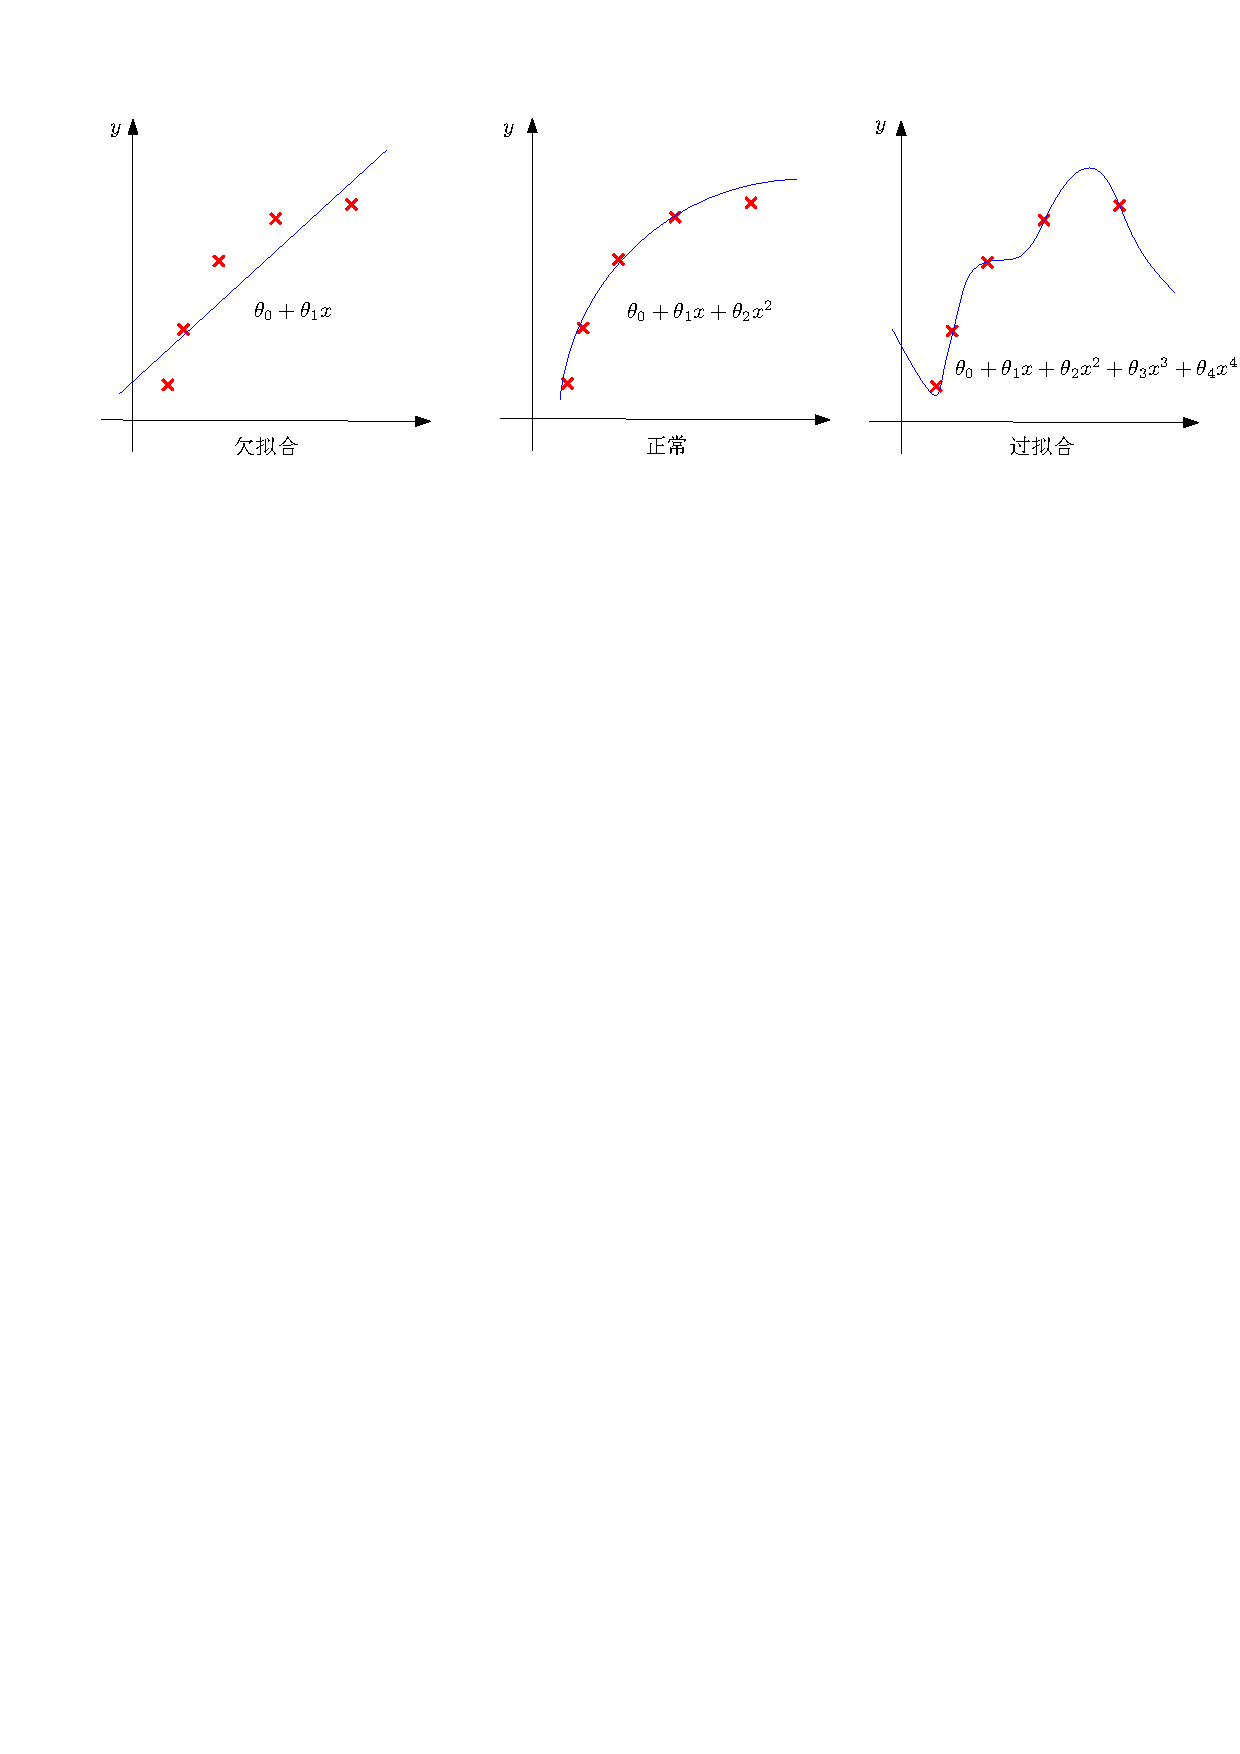
\includegraphics[width=0.85\textwidth]{fit.pdf}
	\caption{拟合情况}
	\label{overfit}
\end{figure}


一个好的模型不仅应当对已有的训练样本拟合的很好, 还应该对未知数据有很好的预测能力(这一般称为模型的泛化能力), 否则我们得到这个模型也没有太大实际意义. 如果模型太复杂, 可能对训练样本表现不错, 但预测能力差, 这在机器学习的很多模型中都能见到, 所以我们要限制模型的复杂度, 避免过度拟合数据或者噪音.

在线性回归中, 模型参数$\bm{\theta}$一定程度上反映了模型的复杂度, 因此我们一般是对参数$\bm{\theta}$施加惩罚, 这种思想我们在数值优化中也多次接触过.

常见的惩罚有$L_{1}$和$L_{2}$惩罚, 分别称为 Lasso Regression 和 Ridge Regression.

所谓 Ridge Regression, 就是使得下式最小
\begin{equation}\label{ridge}
\frac{1}{2} \sum_{i=1}^{m} (y^{(i)} - \bm{\theta}^{T} \bm{x}^{(i)})^2  + \alpha \sum_{j=1}^{n} \theta_{j}^{2} = \frac{1}{2} ||\bm{X} \bm{\theta} -\bm{y}||_{2}^{2} + \alpha ||\bm{\theta}||_{2}^{2}
\end{equation}

注意我们不需要对$\theta_0$做惩罚, 所以上式右边的求和中$j$是从$1$到$n$, 而不是从$0$到$n$(不过最后实际计算时差别影响不大, 所以简写为范数时也就写为了$\bm{\theta}$). 为什么这样能够达到正则化的目的呢? 其实在优化中已经多次提到过这种思想, 这里再说明一下.

比如上面的散点模型可以用二次曲线拟合, 但是我们加了两个特征$x^3$和$x^4$, 那为了让这两个特征几乎不起作用, 我们对它们的系数$\theta_3$和$\theta_4$施加大的惩罚, 即乘以一个非常大的数, 比如 10000, 也就是极小化下式
\begin{equation*}
\frac{1}{2} \sum_{i=1}^{m} (y^{(i)} - \bm{\theta}^{T} \bm{x}^{(i)})^2 + 10000 \theta_{3}^{2} + 10000 \theta_{4}^{2}
\end{equation*}

那么为了求得上式的最小值, $\theta_3$和$\theta_4$只能“牺牲”一下, 或者说“被逼”的, 近似等于$0$了, 这样模型就近似是二次的, 也就达到了避免过拟合的目的.

继续回到(\ref{ridge})式, 要求出它的最小值, 同样可以借助矩阵求导, 直接对$\bm{\theta}$求梯度, 并令其为$0$, 可以得到
\begin{equation*}
\bm{X}^{T} \bm{X} \bm{\theta} - \bm{X}^{T} \bm{y} + \alpha \bm{\theta} = 0
\end{equation*}

于是可得估计为
\begin{equation*}
\bm{\theta} = (\bm{X}^{T} \bm{X} + \alpha I)^{-1} \bm{X}^{T} \bm{y}
\end{equation*}

当$\alpha$充分大的时候, 必然能使惩罚参数近似为$0$, 相当于矩阵$\bm{X}^{T} \bm{X} + \alpha I$一定正定, 这不正是我们之前讨论过正规方程组系数矩阵不正定的情况吗? 所以, 我们当时给系数矩阵加上了$\alpha I$是有道理的, 它居然还能避免过拟合, 想想真是好!

当然, 真正求解 Ridge Regression, 肯定也不会用解方程组的办法, 而是用优化中的各种迭代法, 也就还是梯度下降法、牛顿法等等, 这里的梯度求法和基本线性回归的一样, 就不再写出了.

所谓 Lasso Regression, 与 Ridge Regression 的区别在于施加的是$L_{1}$惩罚, 即使得下式最小
\begin{equation*}
\frac{1}{2}  \sum_{i=1}^{m} (y^{(i)} - \bm{\theta}^{T} \bm{x}^{(i)})^2  + \alpha \sum_{j=1}^{n} |\theta_{j}| = \frac{1}{2}||\bm{X} \bm{\theta} -\bm{y}||_{2}^{2} + \alpha ||\bm{\theta}||_{1}
\end{equation*}

其中$\alpha$也是惩罚参数. Lasso Regression 能够正则化的原因同 Ridge Regression 是一样的, 毕竟只是换了个范数嘛, 那他们有什么区别呢?

首先, 一个大的区别就是$L_{1}$范数不容易处理, 这我们再很多数学课都非常熟悉了, 所以 Lasso Regression 无法得出解的精确表达式, 只能借助优化办法进行数值计算.

其次, 这涉及到$L_{1}$范数和$L_{2}$范数的本质不同. 如果测试过数据你会发现, 用$L_{2}$范数得到的参数估计值可能都比较小, 但用$L_{1}$范数的话, 会发现很多参数的估计值为$0$, 也就是得到的解比较稀疏. 这样当特征维数比较高的时候非常有用. 这是为什么呢? 直观展示可见下图
\begin{figure}[!htb]
	\centering
	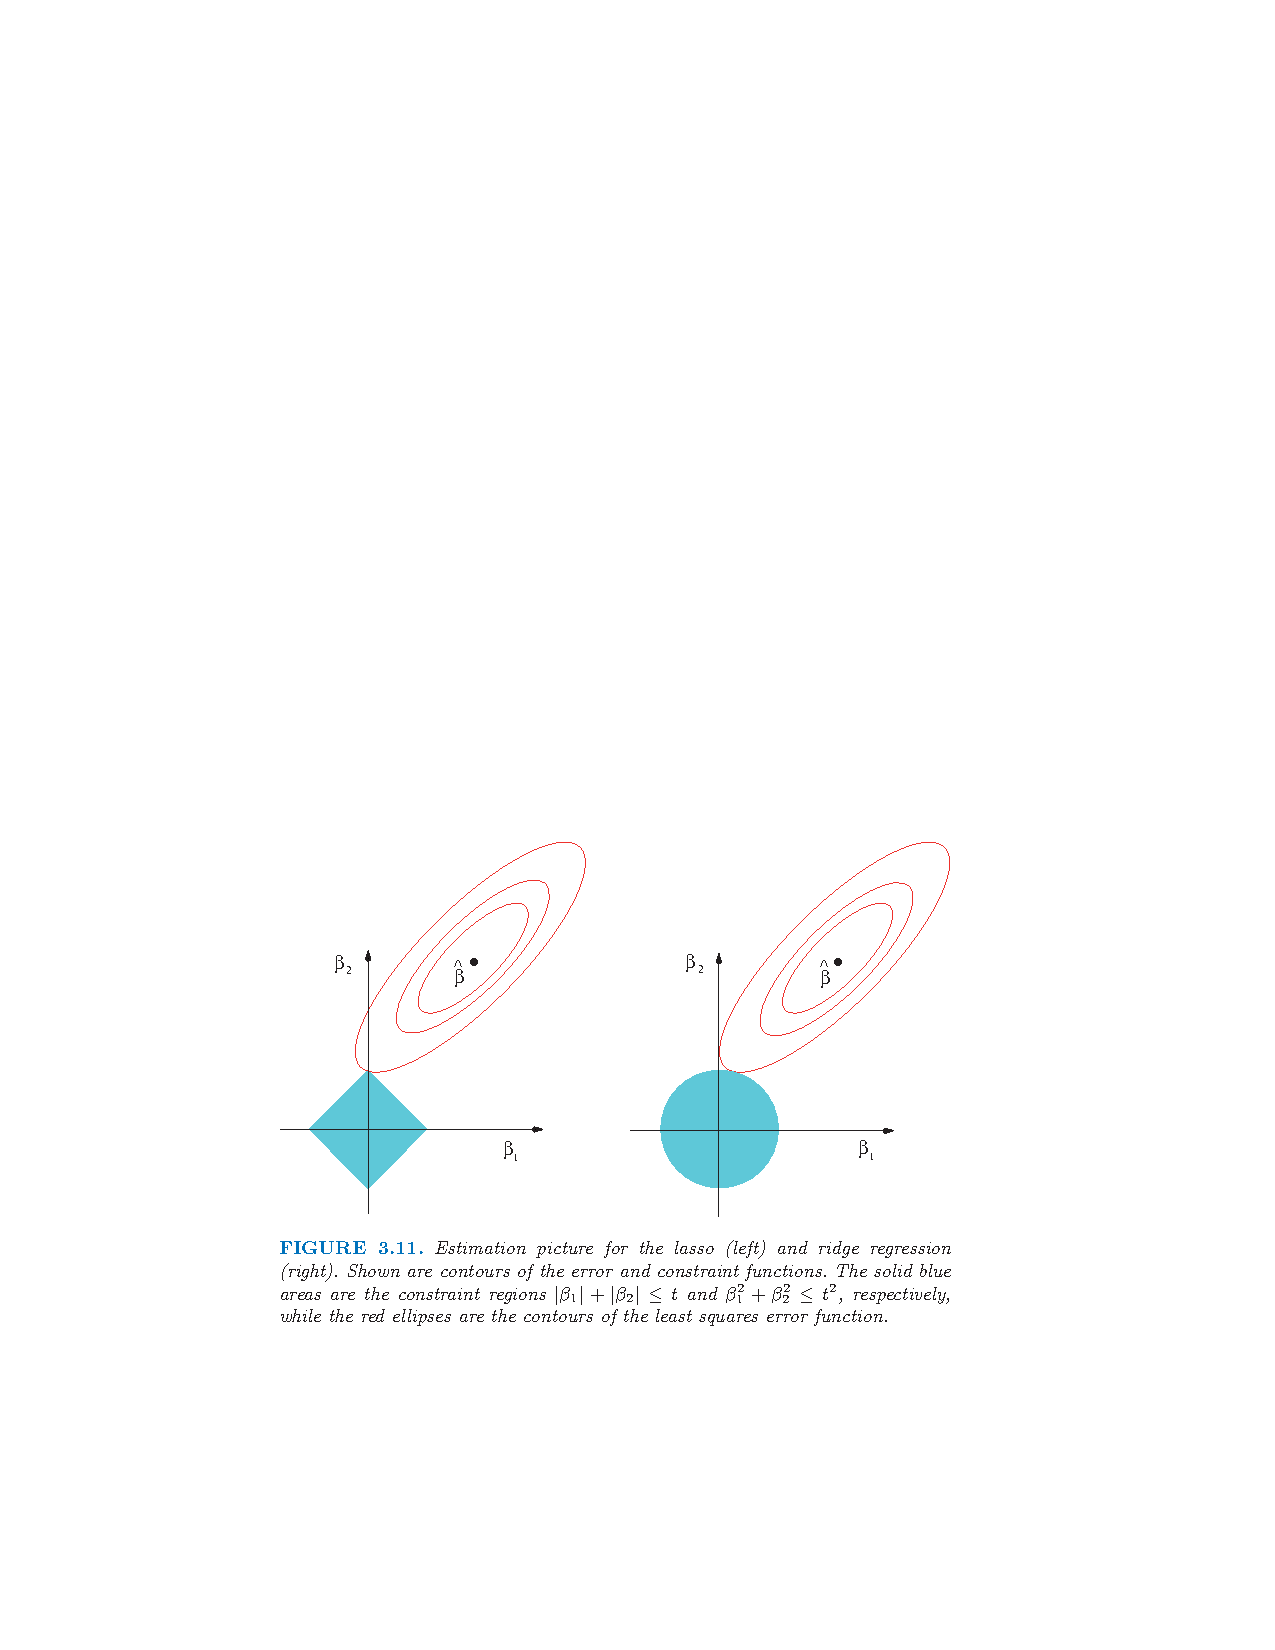
\includegraphics[width=0.80\textwidth]{norm.pdf}
	\caption{Ridge and Lasso}
	\label{norm}
\end{figure}

该图来自 ESL 的第三章, 关于 Ridge VS Lasso 很多文献中都有大篇幅讨论, 这里就不再多述了.

最后提一下 Elastic Net, 它是把 Ridge 和 Lasso 综合到了一块, 即极小化下式
\begin{equation*}
\frac{1}{2m} ||\bm{X} \bm{\theta} - \bm{y}||_{2}^{2} + \alpha \left[ \rho ||\bm{\theta}||_{1} + \frac{1 - \rho}{2} ||\bm{\theta}||_{2}^{2}  \right] 
\end{equation*}
  
其中$\alpha$是惩罚参数, 而$\rho$调整 Ridge 和 Lasso 的比重. Python 的 sklearn 包和 R 的 glmnet 包都能提供以上正则化模型的计算方法. 事实上, 正则化还涉及到了变量选择或者说模型选择的问题, 这就是一个更大的问题了, 可参考其他文献.



\section{统计角度 VS 机器学习}
以上大都是从机器学习的角度来看问题, 主要的目的是估计出参数$\bm{\theta}$, 至于预测效果与模型选择等, 可由训练误差与测试误差决定.

这里我们要注意一个问题, 即统计方法和机器学习方法的异同. 从经典统计学的角度看, 参数$\bm{\theta}$是一个未知的固定常数, 但是估计量$\hat{\bm{\theta}}$是一个随机变量, 是随机样本的函数, 因此, 经典统计学会进一步分析估计量的统计性质, 比如分布等等, 进而寻求参数的区间估计, 或者对我们的结果进行假设检验, 比如模型系数的显著性检验, 以及利用 AIC 准则或者 BIC 准则进行模型选择等等. 而在机器学习的框架中, 虽然也会借助统计方法构建模型, 但重点不在于那些假设检验, 机器学习有自己的模型选择方法.

另外一方面, 从贝叶斯统计的角度看, 一切未知量都是随机变量, 即参数$\bm{\theta}$不是一个未知的常数, 它也是一个随机变量, 只要我们给它一个合适的先验分布, 然后计算出后验分布, 也可进行各种统计推断, 而且往往比经典统计学更合理一些, 比如上面的最大似然估计会过拟合, 因此需要加上惩罚项来正则化, 而我们很容易证明, 假如$\bm{\theta}$的先验分布是 Laplace 分布, 即$p(\bm{\theta})  = (\alpha / 2)^{n} \exp (-\alpha ||\bm{\theta}||_{1})$, 其中常数$\alpha > 0$, 则$\bm{\theta}$的最大后验估计由下式给出:
\begin{equation*}
\min_{\bm{\theta}} \left( \sum_{i=1}^{m} - \log p(y^{(i)}|\bm{x}^{(i)};\bm{\theta}) + \alpha ||\bm{\theta}||_{1} \right)
\end{equation*}

这恰好即为$L_{1}$正则化. 因此, 运用贝叶斯统计的观点来看问题, 能自动避免过拟合, 接下来我们就来看如何用贝叶斯方法进行线性回归.



\section{贝叶斯线性回归}
在贝叶斯统计中, 关键是要求出后验分布, 一般利用核方法, 即
\begin{equation*}
p(\bm{\theta} | \bm{x}) \propto p(\bm{\theta}) \cdot p(\bm{x} | \bm{\theta}) = p(\bm{\theta}) \cdot L(\bm{\theta} | \bm{x}) = K(\bm{\theta})
\end{equation*}

其中$L(\bm{\theta} | \bm{x})$就是样本似然函数$L(\bm{\theta})$, 最大后验估计即要使$K(\bm{\theta}) = p(\bm{\theta}) \cdot L(\bm{\theta | x})$最大. 注意在线性回归中, 这里的$p(\bm{\theta} | \bm{x})$应当理解为$p(\bm{\theta} | \bm{x}, y)$, 因为本质上$\bm{x}, y$合在一起是一组样本.

前面已经求得
\begin{equation*}
p(\bm{x} | \bm{\theta}) = L(\bm{\theta} | \bm{x}) = L(\bm{\theta}) = \prod_{i=1}^{m} p(y^{(i)} | \bm{x}^{(i)}; \bm{\theta})
\end{equation*}

下面来看$\bm{\theta}$的先验分布$p(\bm{\theta})$.

假定$\bm{\theta}$的先验分布为 Laplace 分布, 即
\begin{equation*}
p(\bm{\theta}) = \left( \frac{\alpha}{2} \right)^{n} \mathrm{e}^{-\alpha ||\bm{\theta}||_{1}}
\end{equation*}

其中$\alpha > 0$为常数, 则有
\begin{equation*}
K(\bm{\theta}) = p(\bm{\theta}) \cdot p(\bm{x | \theta}) = \left(\frac{\alpha}{2} \right)^{n} \mathrm{e}^{-\alpha ||\bm{\theta}||_{1}} \cdot \prod_{i=1}^{m} p(y^{(i)}|\bm{x}^{(i)}; \bm{\theta})
\end{equation*}

对$K(\bm{\theta})$取负对数, 可得
\begin{equation*}
-\log K(\bm{\theta}) = - n \log \frac{\alpha}{2} + \alpha ||\bm{\theta}||_{1} - \sum_{i=1}^{m} \log p(y^{(i)}|\bm{x}^{(i)};\bm{\theta})
\end{equation*}

极大化$K(\bm{\theta})$与极小化$-\log K(\bm{\theta})$是一样的, 即等价于
\begin{equation*}
\min_{\bm{\theta}} \left( \sum_{i=1}^{m} - \log p(y^{(i)}|\bm{x}^{(i)};\bm{\theta}) + \alpha ||\bm{\theta}||_{1} \right)
\end{equation*}

这就是$L_{1}$正则化, 于是我们就得到了前面所说的结果.

此外, 如果假定$\theta_j$的先验分布为
\begin{equation*}
\theta_{j} \sim N(0,s^{2}) = \frac{1}{\sqrt{2 \pi} s} \mathrm{e}^{-\frac{\theta_{j}^{2}}{2s^2}} , j = 1,2,\cdots n
\end{equation*}

于是可得$\bm{\theta}$的先验分布为
\begin{equation*}
p(\bm{\theta}) = \prod_{j=1}^{n} \frac{1}{\sqrt{2 \pi} s} \mathrm{e}^{-\frac{\theta_{j}^{2}}{2s^2}} = \left( \frac{1}{\sqrt{2 \pi} s} \right)^{n} \mathrm{e}^{-\frac{\bm{\theta}^{T} \bm{\theta}}{2s^2}}
\end{equation*}

进一步有
\begin{equation*}
K(\bm{\theta}) = p(\bm{\theta}) \cdot p(\bm{x | \theta}) = \left( \frac{1}{\sqrt{2 \pi} s} \right)^{n} \mathrm{e}^{-\frac{\bm{\theta}^{T} \bm{\theta}}{2s^2}} \cdot \prod_{i=1}^{m} p(y^{(i)}|\bm{x}^{(i)};\bm{\theta})
\end{equation*}

还是对$K(\bm{\theta})$取负对数, 可得极小化$- \log K(\bm{\theta})$即为
\begin{equation*}
\min_{\bm{\theta}} \left( \sum_{i=1}^{m} - \log p(y^{(i)}|\bm{x}^{(i)};\bm{\theta}) + \frac{\bm{\theta}^{T} \bm{\theta}}{2s^2} \right)
\end{equation*}

注意到$\bm{\theta}^{T} \bm{\theta} = ||\bm{\theta}||_{2}^{2}$, 因此这相当于$L^{2}$正则化.

以上正态分布的假定相当于$\bm{\theta} \sim \mathcal{N}(\bm{0}, s^{2}\bm{I})$. 当然, 我们也可以假定$\bm{\theta}$的先验分布为其他的形式, 比如$\mathcal{N}(\bm{\mu}, \bm{S})$, 只不过处理会稍微复杂些, 这里就先不讨论了. 此外, 这里假定超参数比如$s$是已知的, 如果$s$未知, 我们也可以给$s$一个分布, 只不过讨论会更麻烦些.

这里我们看到, 从贝叶斯统计的观点看, 正则化相当于给参数$\bm{\theta}$赋予先验信息而已. Ridge Regression 相当于先验分布是正态分布, 而 Lasso Regression 相当于先验分布是 Laplace 分布.


\section{变分贝叶斯线性回归}
\subsection{变分贝叶斯一般框架}
在变分贝叶斯中, 我们将所有观测到的样本记为$\bm{X}$, 不妨设有$m$个样本, 即有$\bm{X} = \{ \bm{x}^{(1)}, \bm{x}^{(2)}, \cdots, \bm{x}^{(m)} \}$, 把所有的未知参数和隐变量(latent variable)记为$\bm{Z}$, 我们的目的是要估计出后验分布$p(\bm{Z} | \bm{X})$, 有了这个后验分布, 我们就可以估计出未知参数了.

但是解析的算出后验分布$p(\bm{Z} | \bm{X})$的表达式是几乎不可能的, 我们考虑用一个分布$q(\bm{Z})$去近似它. 为此先来看一个关系.
\begin{align*}
\ln p(\bm{X}) & = \ln \frac{p(\bm{X}, \bm{Z})}{p(\bm{Z} | \bm{X})}  = \int q(\bm{Z}) \ln \frac{p(\bm{X}, \bm{Z})}{p(\bm{Z} | \bm{X})} \diff \bm{Z} \\
& = \int q(\bm{Z}) \ln \left( \frac{p(\bm{X}, \bm{Z})}{p(\bm{Z} | \bm{X})} \cdot \frac{q(\bm{Z})}{q(\bm{Z})} \right) \diff \bm{Z} \\
& = \int q(\bm{Z}) \left( \ln \frac{q(\bm{Z})}{p(\bm{Z} | \bm{X})} + \ln \frac{p(\bm{X}, \bm{Z})}{q(\bm{Z})} \right) \diff \bm{Z} \\
& = \int q(\bm{Z}) \cdot \ln \frac{q(\bm{Z})}{p(\bm{Z} | \bm{X})} \diff \bm{Z} + \int q(\bm{Z}) \cdot \ln \frac{p(\bm{X}, \bm{Z})}{q(\bm{Z})} \diff \bm{Z} \\
& = - \int q(\bm{Z}) \cdot \ln \frac{p(\bm{Z} | \bm{X})}{q(\bm{Z})} \diff \bm{Z} + \int q(\bm{Z}) \cdot \ln \frac{p(\bm{X}, \bm{Z})}{q(\bm{Z})} \diff \bm{Z} \\
& = \mathrm{KL}(q||p) + \mathcal{L}(q)
\end{align*}

其中$\mathrm{KL}(q || p)$表示$q(\bm{Z})$与$p(\bm{Z} | \bm{X})$间的 KL 散度.
\begin{equation*}
\mathrm{KL}(q || p) = - \int q(\bm{Z}) \cdot \ln \frac{p(\bm{Z} | \bm{X})}{q(\bm{Z})} \diff \bm{Z} \geqslant 0
\end{equation*}

从这个角度看, $\mathrm{KL}(q || p)$反映了我们用$q(\bm{Z})$去近似$p(\bm{Z} | \bm{X})$的差距, 这个值越小越好, 而且我们知道$\mathrm{KL}(q || p) = 0 \Longleftrightarrow q(\bm{Z}) = p(\bm{Z} | \bm{X})$.

在这里, 我们是通过不断最大化$\mathcal{L}(q)$来达到相同的目的, 而$\mathcal{L}(q)$刚好是一个函数$q(\bm{Z})$的泛函, 变分的名称由此得来.

如同一般的变分法, 这里要对$q(\bm{Z})$做某些要求, 相当于把$q(\bm{Z})$限制到某个空间中. 假设$\bm{Z}$可独立成$M$个部分$Z_{i}, i = 1,2,\cdots,M$, 那么最常用的一个要求是因子分解分布, 即有
\begin{equation*}
q(\bm{Z}) = \prod_{i=1}^{M} q_{i}(Z_{i})
\end{equation*}

在此限定条件下我们来求$\mathcal{L}(q)$的最大值, 总体思路是把$\mathcal{L}(q)$拆分成独立的$q_{j}(Z_{j})$, 从而对每一项求最大值, 以下推导中将$q_{j}(Z_{j})$简记为$q_{j}$, 于是有
\begin{align*}
\mathcal{L}(q) & = \int q(\bm{Z}) \cdot \ln \frac{p(\bm{X}, \bm{Z})}{q(\bm{Z})} \diff \bm{Z} \\
& = \int \prod_{i} q_{i}(Z_{i}) \left( \ln p(\bm{X}, \bm{Z}) - \ln \prod_{i}q_{i}(Z_{i}) \right) \diff \bm{Z} \\
& = \int \prod_{i} q_{i} \left( \ln p(\bm{X}, \bm{Z}) - \sum_{i} \ln q_{i} \right) \diff \bm{Z} \\
& = \int \prod_{i} q_{i} \ln p(\bm{X}, \bm{Z}) \prod_{i} \diff Z_{i} - \sum_{i} \int \prod_{j} q_{j} \ln q_{i} \diff Z_{i} \\
& = \int q_{j} \left( \ln p(\bm{X}, \bm{Z}) \prod_{i \neq j} (q_{i} \diff Z_{i}) \right) \diff Z_{j} - \int q_{j} \ln q_{j} \diff Z_{j} - \sum_{i \neq j} \int q_{i} \ln q_{i} \diff Z_{i} \\
& = \int q_{j} \ln \tilde{p}(\bm{X},Z_{j}) \diff Z_{j} - \int q_{j} \ln q_{j} \diff Z_{j} - \sum_{i \neq j} \int q_{i} \ln q_{i} \diff Z_{i} \\
& = - \int q_{j} \ln \frac{\tilde{p}(\bm{X},Z_{j})}{q_{j}} \diff Z_{j} - \sum_{i \neq j} \int q_{i} \ln q_{i} \diff Z_{i} \\
& = - \mathrm{KL}(q_{j} || \tilde{p}) - \sum_{i \neq j} \int q_{i} \ln q_{i} \diff Z_{i}
\end{align*}

其中
\begin{equation*}
\ln \tilde{p}(\bm{X}, Z_{j}) = \int \ln p(\bm{X}, \bm{Z}) \prod_{i \neq j} (q_{i} \diff Z_{i}) = \mathbb{E}_{i \neq j}[\ln p(\bm{X}, \bm{Z})]
\end{equation*}

显然, 当$\mathrm{KL}(q_{j} || \tilde{p}) = 0$时上式取得最大值, 也即$q_{j}(Z_{j}) = \tilde{p}(\bm{X}, Z_{j})$, 因此最优分布$q_{j}^{*}(Z_{j})$即为
\begin{equation*}
\ln q_{j}^{*}(Z_{j}) = \ln \tilde{p}(\bm{X}, Z_{j}) = \mathbb{E}_{i \neq j}[\ln p(\bm{X}, \bm{Z})] + \textrm{const}
\end{equation*}

这里的常数是为了保证分布$q_{j}^{*}(Z_{j})$的正则性, 直接进行归一化可得
\begin{equation*}
q_{j}^{*}(Z_{j}) = \frac{\exp(\mathbb{E}_{i \neq j}[\ln p(\bm{X}, \bm{Z})])}{\displaystyle \int \mathrm{exp}(\mathbb{E}_{i \neq j}[\ln p(\bm{X}, \bm{Z})]) \diff Z_{j}}
\end{equation*}

这便是最优分布的表达式.

关于变分贝叶斯还有很多东西, 这里就不再讨论了.




\subsection{变分贝叶斯线性回归}






\section{总结}






\newpage

\section*{附录}








\end{document}